%%%%%%%%%%%%%%%%%%%%%%%%%%%%%%%%%%%%%%%%%%%%%%%%%%%%%%%%%%%%%%%%%%%%%%%%%%%%%%%%%%%%%%%%%%%%%%%%%%%%%%
%
%   Filename    : chapter_1.tex 
%
%   Description : This file will contain your Research Description.
%                 
%%%%%%%%%%%%%%%%%%%%%%%%%%%%%%%%%%%%%%%%%%%%%%%%%%%%%%%%%%%%%%%%%%%%%%%%%%%%%%%%%%%%%%%%%%%%%%%%%%%%%%

\chapter{Introduction}
\label{sec:intro}    %--note: labels help you with hyperlink editing (using your IDE)
%%
%% --- 1.1 Background of the Study --- %%
%%

\section{Background of the Study}
\label{sec:overview}

%
%   NOTE: You have to delete/replace the unnecessary paragraphs with your own text.
%
History is normally taught with traditional methods such as lectures and discussions. As it requires high levels of understanding, the youth often avoids history. There are other methods that lecturers utilize in teaching history, such as creative means like audio-visual presentations, software, and interactive means. Video games provide an excellent example of interactive learning. Not only is it popular among the new generation, but it grants freedom to choose however they may play the game.

\subsection{Students' Hardship in Classes}
There are multiple factors which makes a student lose their interest and participation in a typical classroom settings. Some of the factors include easy or difficult materials, lack of interest in a subject, and a lecture-based environment \cite{medium:mosley}. Out of all the problems which causes the students to disconnect from the act of learning, test-driven classroom culture was one of the biggest factor which significantly impacts students' educational experience \cite{mora}. The students’ negative view of the classroom primarily focused on multiple standardized test they needed to prepare, and how classes were centered around these tests rather than students.

The same study by \cite{mora} showed how students were less bored and engaged when the classes were integrated with more interactive and hands-on activities such as poster-making and science experiments, rather than typical lecture based classroom set ups. This behavior of the students opens up to the possibility of integrating game-based learning material to enhance the involvement of the students to the class and further enhance their performances by creating a student-centered environment.


\subsection{Utilization of Augmented Reality with Affective Learning}
//TODO Write


\begin{comment}
    
\subsection{Popularity of Video Games}

    Video Games are a ubiquitous concept in modern times. Video games have taken over the world in terms of popularity; its scope reaching the whole world in its usage. As of 2022, there are  3.03 Billion players worldwide \cite{enterpriseappstoday2023}. In a specific look,  Steam, one of the biggest video game distributors online has had a rapid rise of player base. From 2012 till December 2020 the average number of players per hour playing through Steam went from around 100 thousand in the first 12 months to 500 thousand on December of 2020 \cite{Mendes2022}. As of 2024, Steam has about 36 Million  peak players, with player numbers never dropping below 20 Million \cite{SteamCharts}.

    With the widespread use and popularity of video games, there were many studies done around video games; aiming to understand how games affect players and how to use or harness video games in other aspects or industries. One of the most promising applications is by combining video games and learning. One of the words connected with education in students is "boring" ; this causes trouble for both students and teachers alike since the feeling of boredom reduces student understanding and motivation \cite{mora}. This lack of understanding and motivation to learn can lead to lesser grades and deteriorating student performance. On the other hand, looking at video games, the opposite is shown. Games are fun, and they are fun due to multiple reasons which adds to the player's immersion and motivation to learn the game and keep playing \cite{malone1980fun}. 

    If one could combine the lackluster environment of school and the addictive fun of video games, then the result would be a way to keep students interested and motivated to learn all while increasing their performance in terms of educational attainment. A guide book has been made for this specifically. "Gaming the Past" is a book teaching teachers how to use video games to supplement history lessons \cite{mccall2022gaming} . One example in the book is using the game "Civilization" to supplement learning resource management through history; the main goal of games, in the book, is to show a different perspective or capture a specific aspect of history that cannot be shown through normal educational materials alone \cite{mccall2022gaming}. This is an amazing discovery that helps both teachers and students in a win-win scenario. This then begs the question, can this concept be studied further?

    

Often times, a graph, illustration, screenshot, or any image can help a reader better understand what we say in text. In academic writing, we call them \textbf{figures}. Please add as many figures as necessary to help build your narrative, but do not go overboard. 

You can add figures in JPG or PNG format as shown in Figure \ref{fig:disneystock}. All figures should also have a descriptive caption. As a general principle, your caption should adequately describe what is shown in the figure, and not just short texts. If we remove all the surrounding text, the reader should still understand what your figure is. 

All figures should be referred to at least once in the surrounding paragraphs. Make sure that you explain what the figure is all about, and that you refer to your figure. You can also use the surround paragraphs to highlight key insights or parts of your figure. For example, \figref{fig:disneystock} shows a graph of the performance of Disney stock from the 1980s to 2012.

%--- the following example shows how to include a figure in PNG format
\begin{figure}[t]                %-- use [t] to place figure at top, [b] to place at the bottom, [h] for here
   \centering                    %-- use this to center the figure
   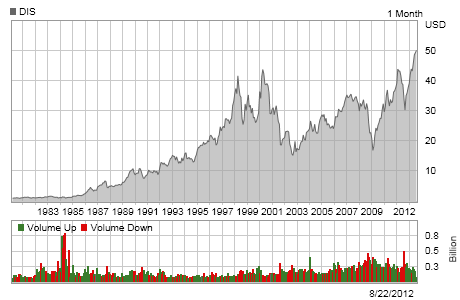
\includegraphics{DisneyChart.png}      %-- include image file named as "disneychart.png" 
   \caption{Disney's stock price chart from the 1980s up to 2012. The top chart shows the stock price in each month. The bottom chart shows the change in volume of transactions. The bars are colored based on the type of movement that happened in a month.}
    \label{fig:disneystock}
\end{figure}

\subsection{Integration of Game-Based Learning in Classroom}
Game-based learning is a method formed from borrowing certain gaming principles and introducing them to real-life scenarios to boost the engagement of students or participants. It allows them to interact with learning materials in a playful, dynamic manner that introduces learning concepts with pre-determined end goals. Usually, it involves incorporating competitiveness, incentives, or taking advantage of feedback loops, which are principles of games. This learning approach allows educational potential by enhancing student's motivation and interest in a subject matter \cite{apho}. 

Game-based learning design allows balance in theoretical content and learning through gaming and explores a targeted learning outcome. Games ensure that students can do repeats without getting bored, and desirable outcomes include cognitive reactions to the interactions received from the game's feedback. It allows a connection between real-life scenarios by connecting the student's understanding of the game to their education \cite{adipat_engaging_2021}.

Studies show that students have improved learning outcomes by using historical games to teach history after engaging with game-based learning materials. According to Najuah et al., the research on the effectiveness of game-based learning, such as educational games, shows a higher difference in student's learning outcomes than those simply using historical animation videos. It has been found that using media in learning builds students' psychology \cite{najuah_effectiveness_2023}. Moreover, according to McCall, digital historical games are a powerful medium to interpret and engage with past scenarios, and teachers found that using games in a classroom setting is helpful \cite{mccall_teaching_2016}. However, using games in a classroom setting reveals that the teacher has to play multiple roles in assisting the students in creating the educational environment. The teacher takes on the additional role of administrator, lecturer, game tutor, and authority for the student to be in the mode of play \cite{markeduc}.

\end{comment}

\begin{comment}
\subsection{Code snippet}

The following shows how to include a program source code (or algorithm). The verbatim environment, as the name suggests, outputs text (including white spaces) as is...

\begin{verbatim}
               #include <stdio.h>
               main()
               {
                    printf("Hello world!\n");
               }
\end{verbatim}
\end{comment}

%%
%% --- 1.2 Research Objectives --- %%
%%
\begin{comment}
\section{Research Objectives}

This subsection states the over--all goal that must be achieved to answer the problem. Address the following: Given your research challenge or opportunity, how do you intend to solve it? What is the main outcome of your research? What kind of contribution do you want to achieve?

The \textbf{general objective} is broken down into three or more specific objectives. The \textbf{specific objectives} are relatively smaller objectives that help you attain your general objective. You can formulate your specific objectives based on your running questions about the project. For example, the group does not have a good picture yet of the different conversation patterns between humans that can be mimicked by conversational agents. A specific objective can be "to identify different human-human conversation patterns." These objectives must be specific, measurable, attainable, realistic, and time-bounded.

Reviewing related literature, studying a particular programming language or development tool (e.g., to study Windows/Object-Oriented/Graphics/C++ programming), and documentation to accomplish the general objective is inherent in all thesis projects and, therefore, must not be included here.


\begin{comment}
%
% IPR acknowledgement: the following sentences and examples are from Ethel Ong's slides 
%     on Research Objectives
%

How to formulate your research objectives:
1. Identify what research steps do you need to perform to achieve your general objective.
2. Identify the questions that must be answered for you to achieve your general objective.
    Thereafter, convert these questions into action statements


Example #1:

Question:
    What strategies do human educators employ in collaborative storytelling with children?

Specific Objective:
   To review existing strategies employed by language educators when sharing storytelling with children


Example #2:

Question:
   How will you represent commonsense knowledge for use by computer systems?

Specific Objective:
   To identify knowledge representation approaches used by existing story generation systems

Example #3:
Question:
   What types of storytelling knowledge are needed to generate stories?

Objective:
    To identify the different types of storytelling knowledge used in generating stories

Example #4:
Question:
    What machine learning approaches will you utilize?

Specific Objective:
    To determine existing machine learning algorithms [that can be used in training the computer system to detect cyberbullying cases] 

Example #5: 
Question:
    How will your research output be evaluated?

Specific Objective:
    To define evaluation metrics for validating the accuracy of the translation
\end{comment}


%
%  The following is the format for presenting your specific objectives; replace them with your own 
%

%%
%% --- 1.3 Scope and Limitations --- %%
%%
\begin{comment}
\section{Scope and Limitations of the Research}
\label{sec:scopelimitations}

This section discusses the boundaries, with respect to the objectives, of the research and the constraints within which the research will be developed. Describe what is and is not included in the scope of your research, supported by your main research question and findings of previous studies. Do not use weak excuses such as the lack of time and/or knowledge to perform the research.

A good rule of thumb is to allocate one paragraph for each of your specific objectives that (1) contains a brief overview of the concept/theory and the purpose of doing the associated objective; and (2) includes a description of the scope/limitation of your study, and followed by brief purpose, rationale and/or justification for your decisions.

The following should also be indicated in your Scope and Limitations (in the appropriate paragraphs matching the objectives, or as a stand-alone paragraph):
\begin{itemize}
   \item The profile and demographics of your target participants
   \item Your data sources (i.e., new data, data from previous studies, data to be provided by some experts, data to be retrieved from social networks)
   \item The specific technology platform to be utilized
   \item The methods for collecting the data
   \item The coverage areas or locations
   \item The duration or time period (e.g., news articles for the year 2016-2017)
\end{itemize}
\end{comment}

%%
%% --- 1.4 Significance of the Research --- %%
%%
\begin{comment}
\section{Significance of the Research}

This section explains why research must be done in this area.  It rationalizes the objective of the research with that of the stated problem. Avoid including sentences such as ``This research will be beneficial to the proponent/department/college'' as this is already an inherent requirement of all BS and MS thesis projects.  Focus on the research's contribution to the Computer Science field.

The following are guide questions that may help your formulate the significance of your research. 


%
% IPR acknowledgement: the following list of items are from Ethel Ong's slides on Significance of the Research
%
\begin{itemize}
\item  What is the relevance and contribution of your work to the computer science community? 

\begin{itemize} 
\item How does your technical contributions or empirical findings advance the field or grow our body of knowledge? 
\item If you built a prototype of an interaction technique, interface, library, tool, or system, what is value does it add compared to existing solutions? 
\end{itemize}

\item What will be your contributions to society in general? 
    \begin{itemize}
      \item How will your main stakeholders benefit from your technical contributions or empirical findings? 
      \item What are the positive social or economic impacts? 
   \end{itemize}
\end{itemize}
\end{comment}

\begin{comment}
If applicable, describe possible commercialization and/or innovation in your research.
\end{comment}

\section{Research Objectives}

\section{Scope and Limitations}

\section{Significance of the Study}